\section{CPU 编程}
Kernel编程最初作为一种 GPU 编程方式而流行。 
随着Kernel编程的普遍化,了解Kernel编程风格如何影响代码到 CPU 的映射非常重要。

CPU 已经发展了很多年。 2005 年左右发生了重大转变,当时时钟速度提高所带来的性能提升逐渐减弱。 
并行性成为受欢迎的解决方案——CPU 生产商没有提高时钟速度,而是引入了多核芯片。 
计算机在同时执行多项任务时变得更加有效!

虽然多核作为提高硬件性能的途径盛行,但要实现软件性能的提升需要付出不小的努力。 
多核处理器要求开发人员提出不同的算法,这样硬件的改进才会引人注目,但这并不总是那么容易。 
我们拥有的核心越多,让它们高效地忙碌就越困难。 
SYCL 是应对这些挑战的编程语言之一,它具有许多有助于利用 CPU(和其他体系结构)上各种形式的并行性的结构。

本章讨论 CPU 架构的一些细节、CPU 硬件通常如何执行 SYCL 应用程序,并提供为 CPU 平台编写 SYCL 代码时的最佳实践。

\subsection{性能注意事项}
SYCL 为并行化我们的应用程序或从头开始开发并行应用程序铺平了一条可移植的路径。 
应用程序在 CPU 上运行时的性能很大程度上取决于以下因素:

\begin{itemize}
	\item Kernel代码启动和执行的底层性能

	\item 在并行Kernel中运行的程序的百分比及其可扩展性

	\item CPU 利用率、有效的数据共享、数据局部性和负载平衡

	\item 工作项之间的同步和通信量

	\item 创建、恢复、管理、挂起、销毁和同步工作项执行的任何线程所引入的开销,
	该开销受串行到并行或并行到串行转换数量的影响

	\item 共享内存引起的内存冲突(包括错误共享内存)

	\item 共享资源(例如内存、写入组合缓冲区和内存带宽)的性能限制
\end{itemize}

此外,与任何处理器类型一样,CPU 可能因供应商而异,甚至因产品一代而异。 
适用于一种 CPU 的最佳实践可能并非适用于其他 CPU 和配置的最佳实践。

\begin{remark}
	要在 CPU 上实现最佳性能,请尽可能多地了解 CPU 架构的特征!
\end{remark}

\subsection{多核 CPU 的基础知识}
多核 CPU 的出现和快速发展推动了共享内存并行计算平台的广泛接受。 
CPU 在笔记本电脑、台式机和服务器级别提供并行计算平台,使其无处不在,几乎无处不在。 
CPU 架构最常见的形式是高速缓存一致性非均匀内存访问 (cc-NUMA),其特点是内存访问时间不完全均匀。 
许多小型双路通用CPU系统都有这种内存系统。 由于处理器中的核心数量以及插槽数量不断增加,这种架构已成为主导。

在 cc-NUMA CPU 系统中,每个插槽连接到系统中总内存的一个子集。 
高速缓存一致性互连将所有套接字粘合在一起,并为程序员提供单一系统内存视图。 
这样的内存系统是可扩展的,因为总内存带宽随着系统中套接字的数量而扩展。 
互连的好处是应用程序可以透明地访问系统中的所有内存,无论数据驻留在何处。 
然而,这是有代价的:从内存访问数据的延迟不再一致(即,我们不再有固定的访问延迟)。 
相反,延迟取决于数据在系统中的存储位置。 在良好的情况下,数据来自直接连接到代码运行的套接字的内存。 
在糟糕的情况下,数据必须来自连接到系统中较远的套接字的内存,
并且由于 cc-NUMA CPU 系统上套接字之间互连的跳数,内存访问的成本可能会增加。

\begin{figure}[H]
	\centering
	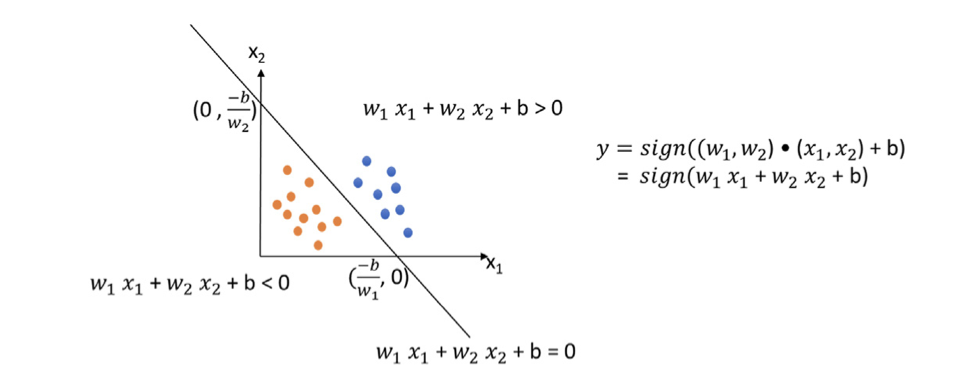
\includegraphics[width=0.9\textwidth]{figs/F16.1.png}
	\caption{\textit{通用多核CPU系统 }}
\end{figure}

图 16-1 显示了具有 cc-NUMA 内存的通用 CPU 架构。 
这是一种简化的系统架构,包含当今通用多插槽系统中的核心和内存组件。 
在本章的其余部分中,该图将用于说明相应代码示例的映射。

为了实现最佳性能,我们需要确保了解特定系统的 cc-NUMA 配置的特征。 
例如,英特尔最新的服务器使用了网状互连架构。 
在此配置中,核心、高速缓存和内存控制器被组织成行和列。 
在努力实现系统的最佳性能时,了解处理器与内存的连接性至关重要。

图 16-1 中的系统有两个插槽,每个插槽有两个Kernel,每个Kernel有四个硬件线程。 
每个核心都有自己的 1 级 (L1) 缓存。 L1 缓存连接到共享的最后一级缓存,该缓存连接到套接字上的内存系统。 
套接字内的内存访问延迟是统一的,这意味着它是一致的并且可以准确预测。

这两个套接字通过缓存一致性互连进行连接。 内存分布在整个系统中,但所有内存都可以从系统中的任何位置透明地访问。 
当访问不在运行访问代码的套接字中的内存时,内存读写延迟是不均匀的,
这意味着从远程套接字访问数据时,它可能会带来更长且不一致的延迟。 
然而,互连的一个关键方面是一致性。 
我们不需要担心整个系统内存中数据的不一致视图,而是可以关注我们访问分布式内存系统的方式对性能的影响。 
更高级的优化(例如,具有宽松内存顺序的原子操作)可以实现不再需要那么多硬件内存一致性的操作,
但是当我们需要一致性时,硬件会为我们提供一致性。

CPU 中的硬件线程是执行工具。 这些是执行指令流的单元。 
图16-1中的硬件线程从0到15连续编号,这是用于简化本章示例讨论的符号。 
除非另有说明,本章中对 CPU 系统的所有引用均指图 16-1 中所示的参考 cc-NUMA 系统。

\subsection{SIMD 硬件基础知识}
1996 年,广泛部署的 SIMD 指令集是 x86 架构之上的 MMX 扩展。 
此后,许多 SIMD 指令集扩展在英特尔架构以及整个行业得到广泛应用。 
CPU Kernel通过执行指令来执行其工作,Kernel知道如何执行的具体指令由指令集(例如 x86、x86\_64、AltiVec、NEON)
和指令集扩展(例如 SSE、AVX、 AVX-512)它实现的。 指令集扩展添加的许多操作都集中在 SIMD 上。

SIMD 指令允许通过使用大于正在处理的数据的基本单位的寄存器和硬件,在单个Kernel上同时执行多个计算。 
例如,使用 512 位寄存器,我们可以使用一条机器指令执行 8 个 64 位计算。

\begin{figure}[H]
	\centering
	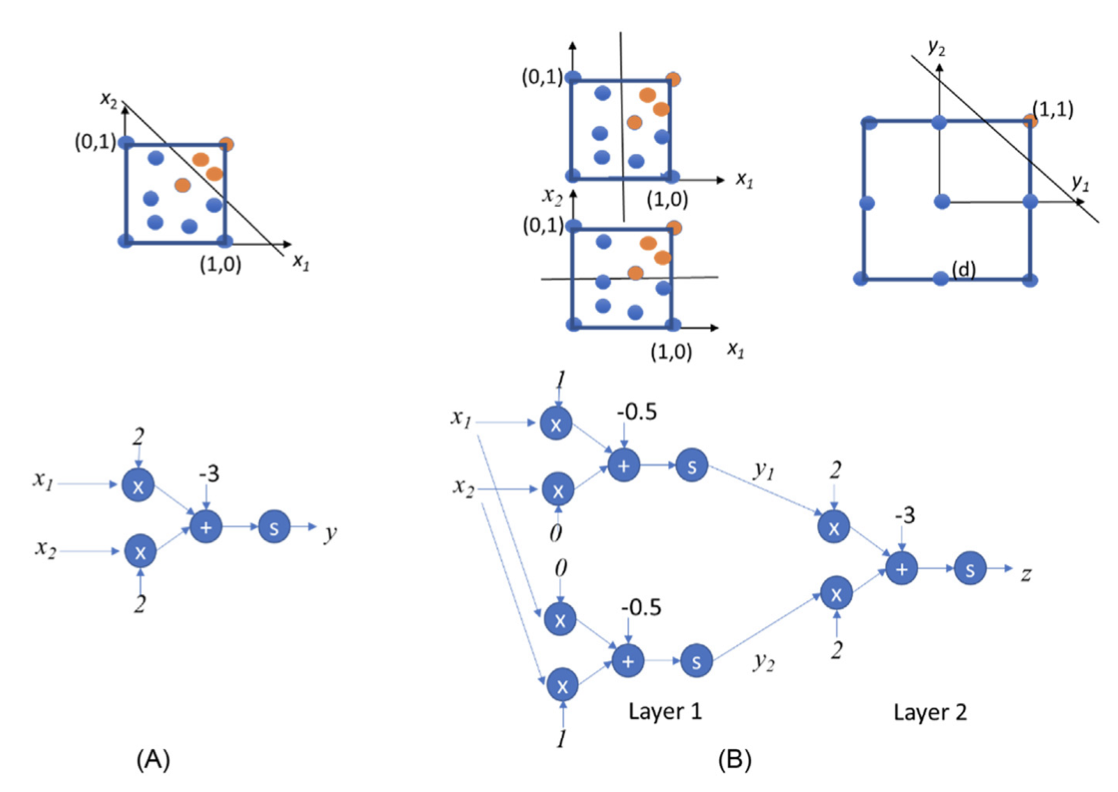
\includegraphics[width=0.9\textwidth]{figs/F16.2.png}
	\caption{\textit{在 CPU 硬件线程中执行 SIMD }}
\end{figure}

理论上,图 16-2 中所示的示例可以使我们的速度提高八倍。 
实际上,它可能会有所缩减,因为八倍加速的一部分用于消除一个瓶颈并暴露下一个瓶颈,例如内存吞吐量。 
一般来说,使用 SIMD 的性能优势因具体场景而异,在少数情况下,
例如广泛的分支发散、非单位步长内存访问的聚集/分散以及 SIMD 加载和存储的缓存行分割,
它可以 甚至比更简单的非 SIMD 等效代码执行得更差。 
也就是说,当我们知道何时以及如何应用(或让编译器应用)SIMD 时,当今的处理器可以实现相当大的收益。 
与所有性能优化一样,程序员应该在将典型目标机器投入生产之前测量其增益。 
本章以下各节提供了有关预期性能提升的更多详细信息。

带有 SIMD 单元的 cc-NUMA CPU 架构构成了多核处理器的基础,
它可以以至少五种不同的方式利用从指令级并行开始的广泛并行性,如图 16-3 所示。

\begin{figure}[H]
	\centering
	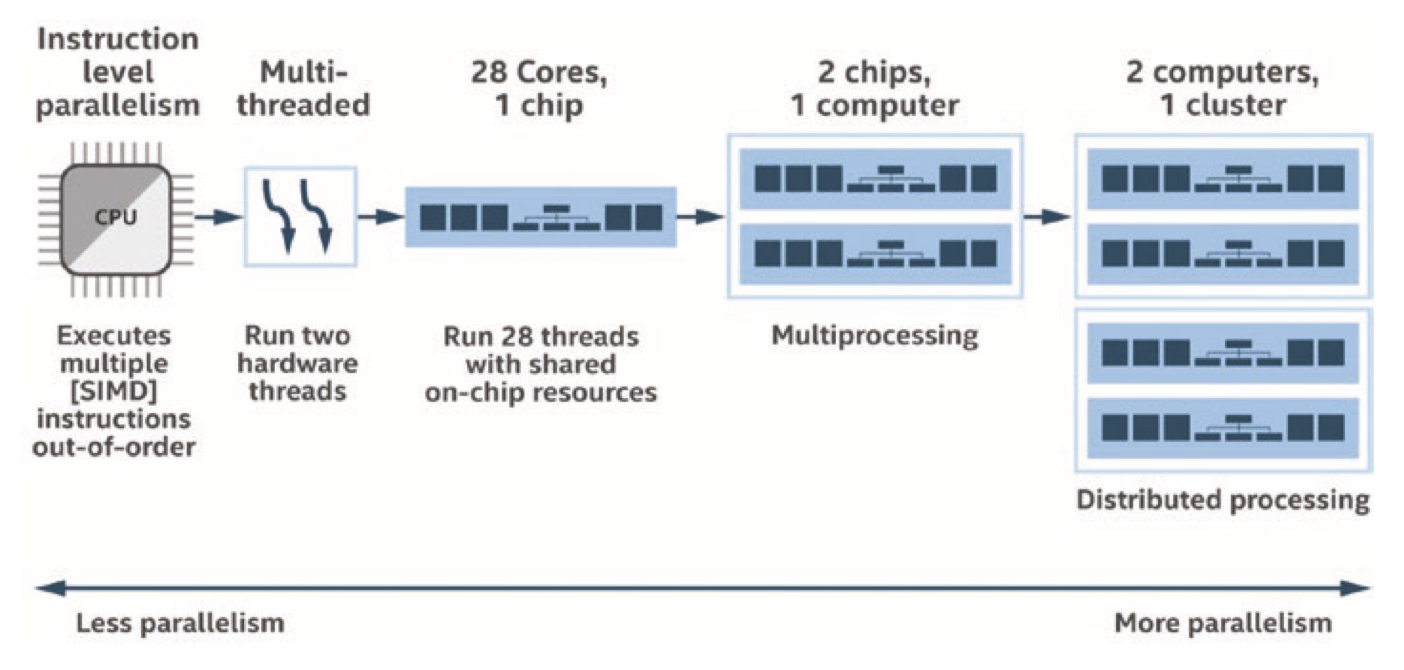
\includegraphics[width=0.9\textwidth]{figs/F16.3.png}
	\caption{\textit{并行执行指令的五种方式 }}
\end{figure}

在图16-3中,指令级并行可以通过单线程内标量指令的乱序执行和SIMD并行来实现。 
线程级并行可以通过在同一核心或不同规模的多个核心上执行多个线程来实现。 
更具体地说,线程级并行性可以从以下方面体现出来:

\begin{itemize}
	\item 现代CPU 架构允许一个核心同时执行两个或多个线程的指令。

	\item 每个处理器内包含两个或多个Kernel的多核架构。 
	操作系统将其每个执行核心视为具有所有关联执行资源的离散处理器。

	\item 处理器(芯片)级别的多处理,可以通过执行单独的代码线程来完成。 
	因此,处理器可以让一个线程从应用程序运行,另一个线程从操作系统运行,或者可以让并行线程从单个应用程序内运行。

	\item 分布式处理,可以通过在计算机集群上执行由多个线程组成的进程来完成,这些进程通常通过消息传递框架进行通信。
\end{itemize}

随着多处理器计算机和多核技术变得越来越普遍,使用并行处理技术作为标准实践来提高性能非常重要。 
本章后面的部分将介绍 SYCL 中的编码方法和性能调优技术,使我们能够在多核 CPU 上实现峰值性能。

与其他并行处理硬件(例如 GPU)一样,为 CPU 提供足够大的数据元素集进行处理非常重要。 
为了演示利用多级并行处理大量数据的重要性,请考虑一个简单的 C++ STREAM Triad 程序,如图 16-4 所示。

\begin{figure}[H]
	\centering
	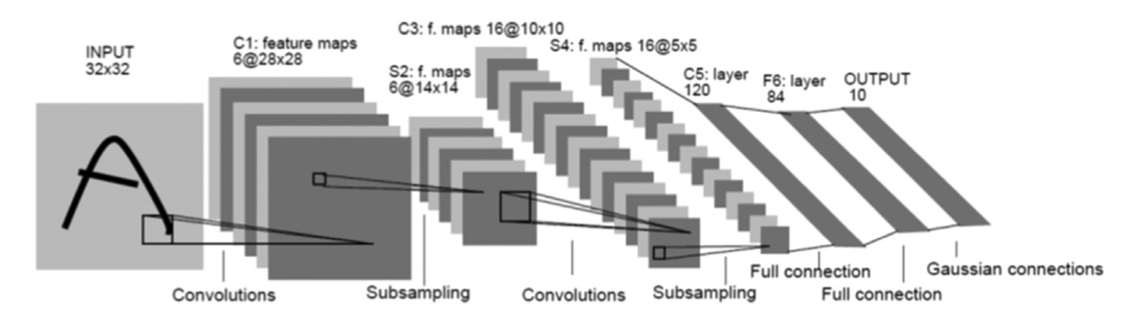
\includegraphics[width=0.9\textwidth]{figs/F16.4.png}
	\caption{\textit{STREAM Triad C++ 循环 }}
\end{figure}

\begin{remark}[STREAM TRIAD WORKLOAD 的说明]
Stream triad workload (www.cs.virginia.edu/stream) 
是 CPU 供应商用来演示内存带宽功能的重要且流行的基准测试工作负载。
我们使用Stream triad Kernel来演示并行Kernel的代码生成,以及通过本章中描述的技术实现显著提高性能的计划方式。
Stream triad是一个相对简单的工作负载,但足以以易于理解的方式显示许多优化。
布里斯托大学有一个流实现,称为Babelstream,其中包括带有sYCL版本的C++。
\end{remark}

STREAM Triad 循环可以在使用单个CPU 核心进行串行执行的CPU 上简单地执行。 
优秀的 C++ 编译器将执行循环向量化,为具有利用指令级 SIMD 并行性的硬件的 CPU 生成 SIMD 代码。 
例如,对于支持 AVX-512 的 Intel Xeon 处理器,Intel C++ 编译器会生成如图 16-5 所示的 SIMD 代码。 
至关重要的是,编译器对代码的转换通过在每次循环迭代中执行更多工作(使用 SIMD 指令和循环展开)减少了循环迭代次数。

\begin{figure}[H]
	\centering
	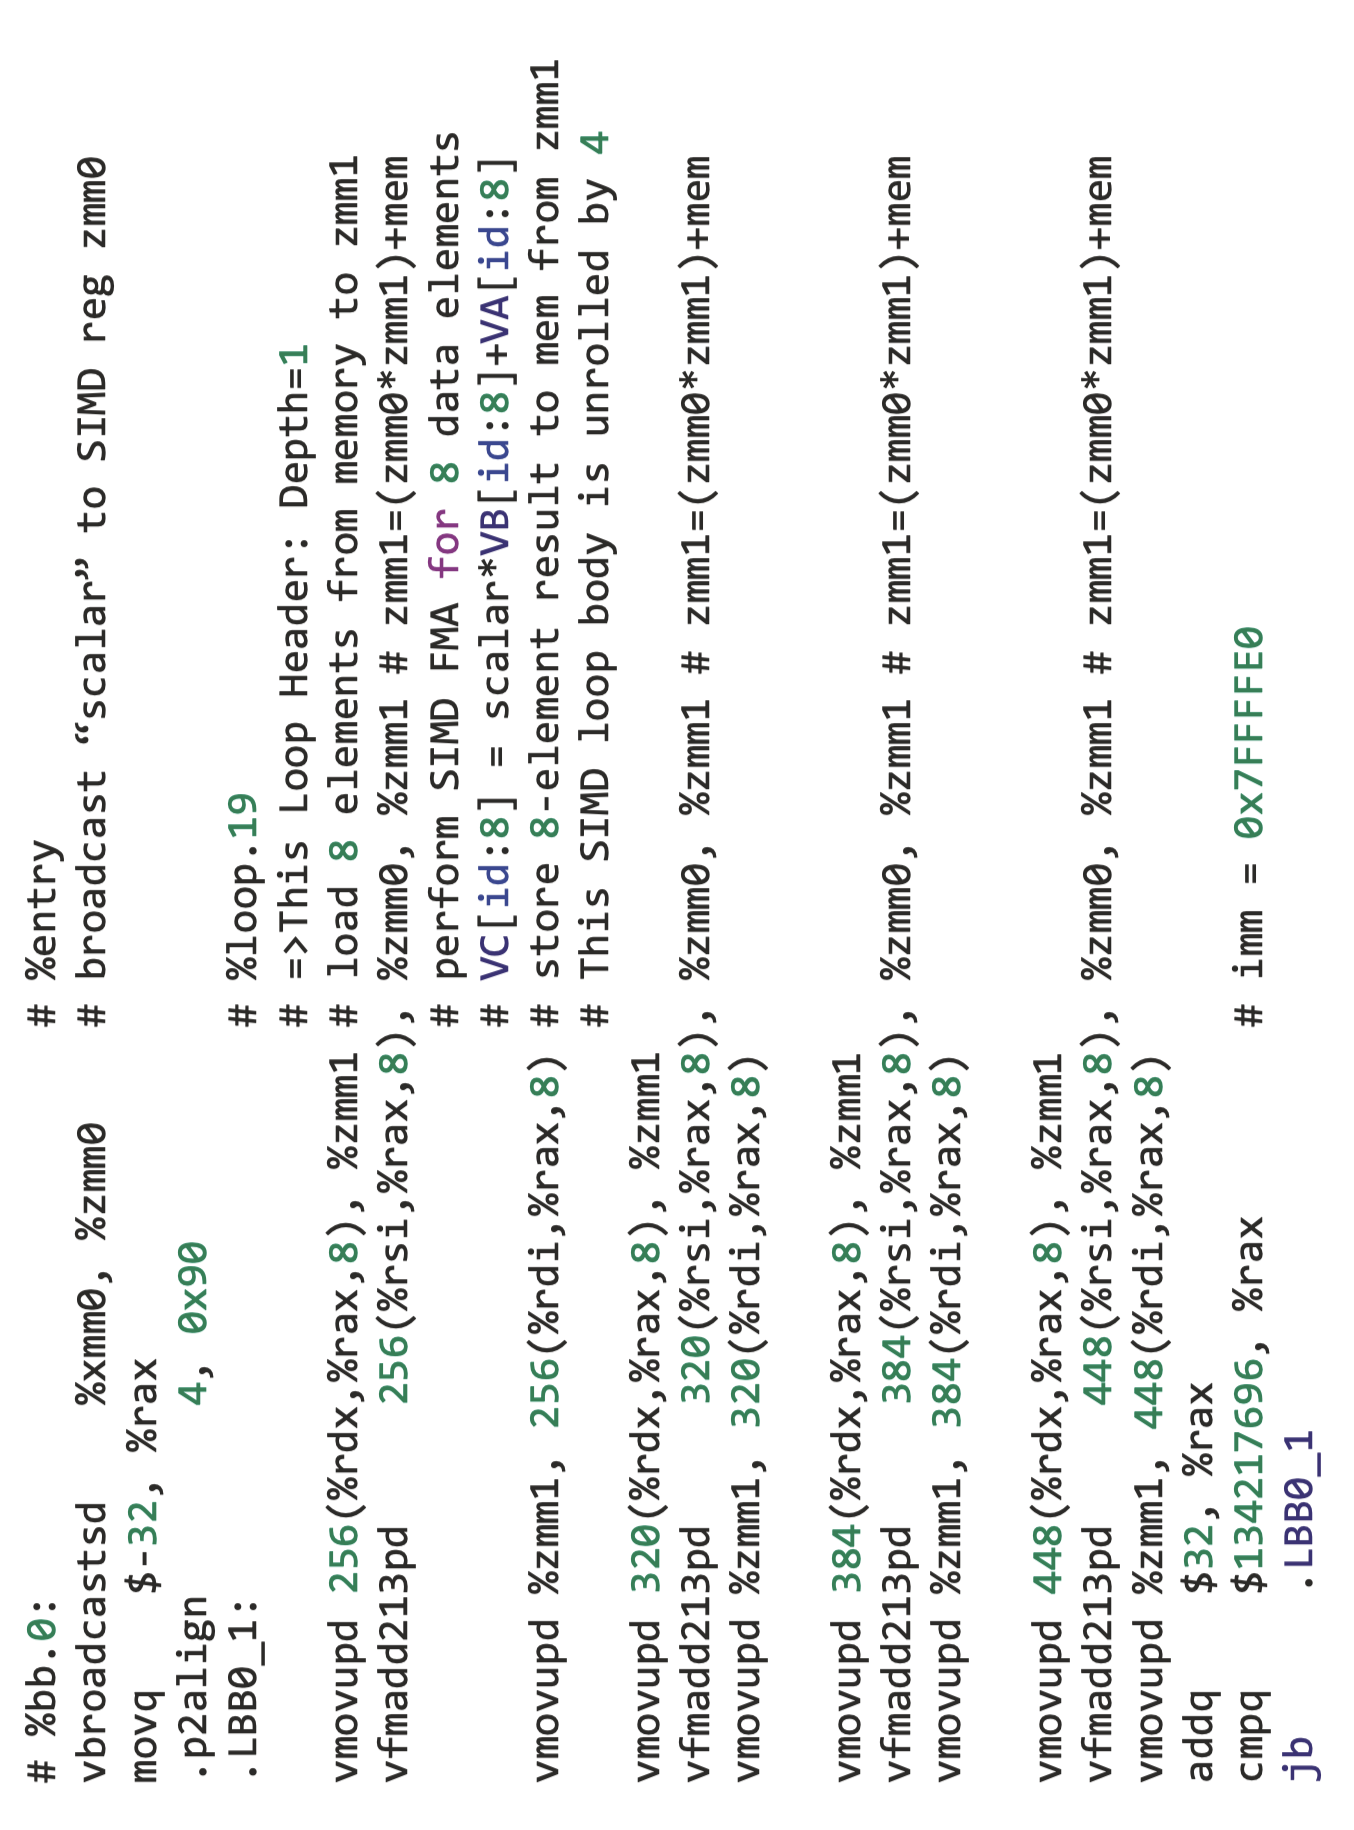
\includegraphics[width=0.9\textwidth]{figs/F16.5.png}
	\caption{\textit{AVX-512 }}
\end{figure}

如果我们尝试在 CPU 上执行此函数,它可能会在较小的数组大小下运行良好,
但效果并不好,因为它不利用 CPU 的任何多核或线程功能。 
然而,如果我们尝试在 CPU 上使用较大的数组大小执行此函数,它的性能可能会非常差,
因为单个线程仅利用单个 CPU 核心,并且当该核心的内存带宽饱和时,就会出现瓶颈。

\subsection{利用线程级并行性}
为了提高 STREAM Triad Kernel的性能,
我们可以通过将循环转换为 parallel\_for Kernel来计算一系列可以并行处理的数据元素。

\begin{figure}[H]
	\centering
	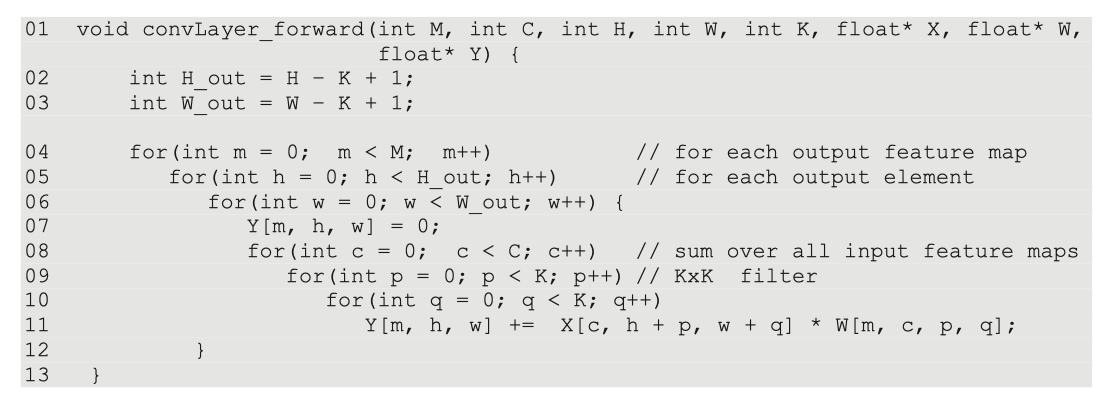
\includegraphics[width=0.9\textwidth]{figs/F16.6.png}
	\caption{\textit{SYCL STREAM Triad parallel\_for Kernel代码 }}
\end{figure}

该 STREAM Triad SYCL 并行Kernel的主体与在 CPU 上以串行 C++ 执行的 STREAM Triad 循环的主体完全相同,
如图 16-6 所示。

\begin{figure}[H]
	\centering
	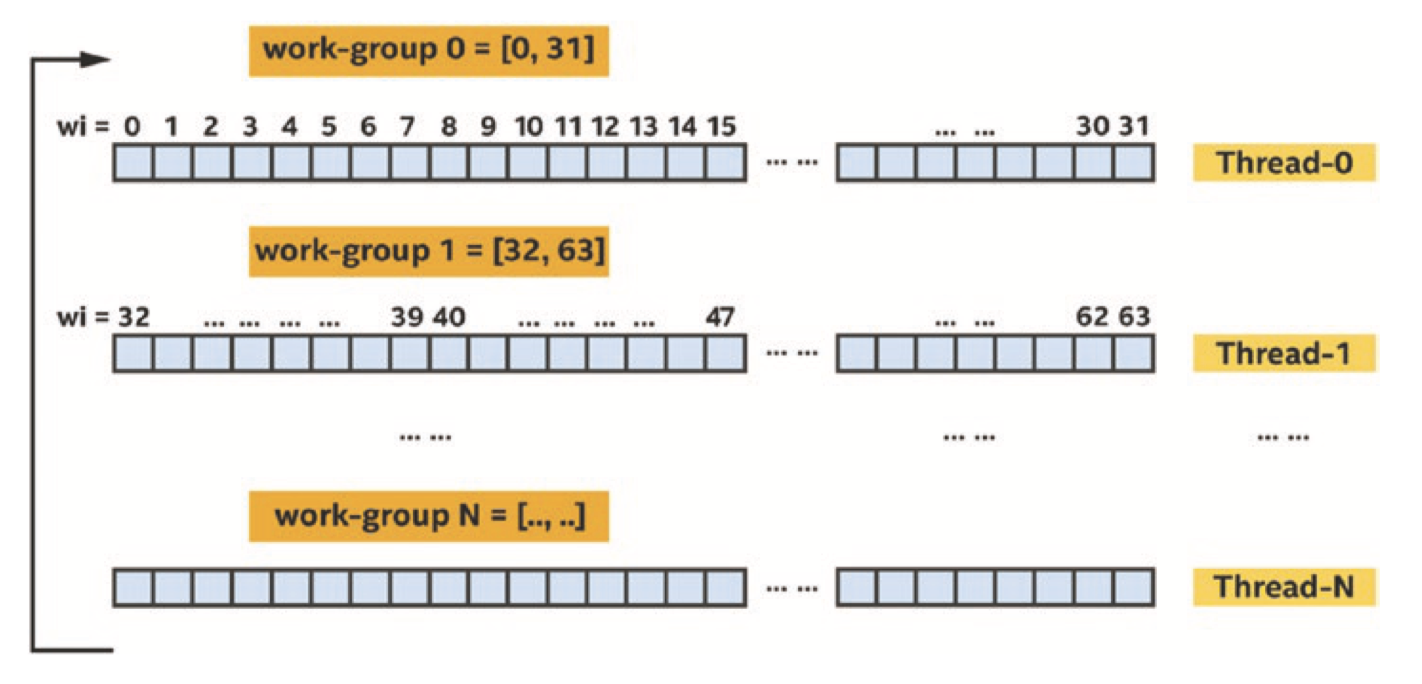
\includegraphics[width=0.9\textwidth]{figs/F16.7.png}
	\caption{\textit{STREAM Triad 并行Kernel的映射 }}
\end{figure}

尽管并行Kernel与使用循环的串行 C++ 编写的 STREAM Triad 函数非常相似,但它的运行速度要快得多,
因为 parallel\_for 允许在多个Kernel上并行处理数组的不同元素。 
图 16-7 显示了如何将该Kernel映射到 CPU。 
假设我们的系统有一个套接字、四个核心,每个核心有两个硬件线程(总共八个线程),
并且该实现在每个包含 32 个工作项的工作组中处理数据。 
如果我们有 1024 个双精度数据元素需要处理,我们将有 32 个工作组。 
工作组调度可以按循环顺序完成,即thread-id = work-group-id mod 8。
本质上,每个线程将执行四个工作组。 每轮可以并行执行八个工作组。 
请注意,在这种情况下,工作组是由 SYCL 编译器和运行时隐式形成的一组工作项。

请注意,在 SYCL 程序中,未指定数据元素被分区并分配给不同处理器核心(或线程)的确切方式。 
这为 SYCL 实现提供了灵活性,可以选择如何最好地在特定 CPU 上执行并行Kernel。 
话虽如此,实现可以为程序员提供某种程度的控制,以实现性能调整(例如,通过编译器选项或环境变量)。

虽然CPU可能会施加相对昂贵的线程上下文切换和同步开销,但在处理器核心上驻留更多软件线程可能是有益的,
因为它为每个处理器核心提供了要执行的工作的选择。 
如果一个软件线程正在等待另一线程产生数据,则处理器核心可以切换到准备运行的不同软件线程,而不会使处理器核心空闲。

\begin{remark}[选择如何绑定和调度线程]
选择一种有效的方案来在线程之间分区和调度工作对于在 CPU 和其他设备类型上调整应用程序非常重要。后续部分将介绍一些技术。
\end{remark}

\subsubsection{线程亲和力洞察}
线程亲和性指定执行特定线程的 CPU 核心。 
如果线程在核心之间移动,性能可能会受到影响,例如,如果线程不在同一核心上执行,
并且数据在不同核心之间来回移动,则缓存局部性可能会变得效率低下。

DPC++ 编译器的运行时库支持多种通过环境变量 DPCPP\_CPU\_CU\_AFFINITY、
DPCPP\_CPU\_PLACES、DPCPP\_CPU\_NUM\_CUS 和 DPCPP\_CPU\_SCHEDULE 将线程绑定到Kernel的方案,
这些方案不是由 SYCL 定义的。 
其他实现可能会公开类似的环境变量。

第一个是环境变量 DPCPP\_CPU\_CU\_AFFINITY。 
使用这些环境变量控件进行调整既简单又成本低,但会对许多应用程序产生巨大影响。 该环境变量的说明如图16-8所示。

\begin{figure}[H]
	\centering
	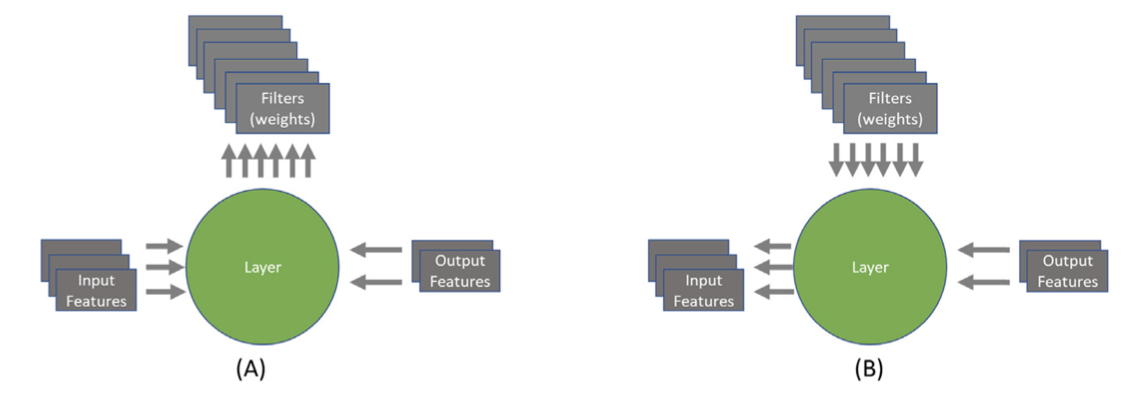
\includegraphics[width=0.9\textwidth]{figs/F16.8.png}
	\caption{\textit{DPCPP\_CPU\_CU\_AFFINITY 环境变量 }}
\end{figure}

当指定环境变量 DPCPP\_CPU\_CU\_AFFINITY 时,软件线程通过以下公式绑定到硬件线程:

spread: boundHT = ( tid mod numHT ) + (tid mod numSocket) × numHT) close: boundHT = tid mod (numSocket × numHT )

其中

\begin{itemize}
	\item tid 表示软件线程标识符

	\item boundHT 表示线程tid 绑定到的硬件线程(逻辑核心)

	\item numHT 表示每个套接字的硬件线程数

	\item numSocket 表示系统中的套接字数量
\end{itemize}

假设我们在双核双插槽系统上运行一个具有八个线程的程序,换句话说,我们有四个核心,总共有八个线程要编程。 
图 16-9 显示了线程如何映射到不同 DPCPP\_CPU\_CU\_AFFINITY 设置的硬件线程和Kernel的示例。

\begin{figure}[H]
	\centering
	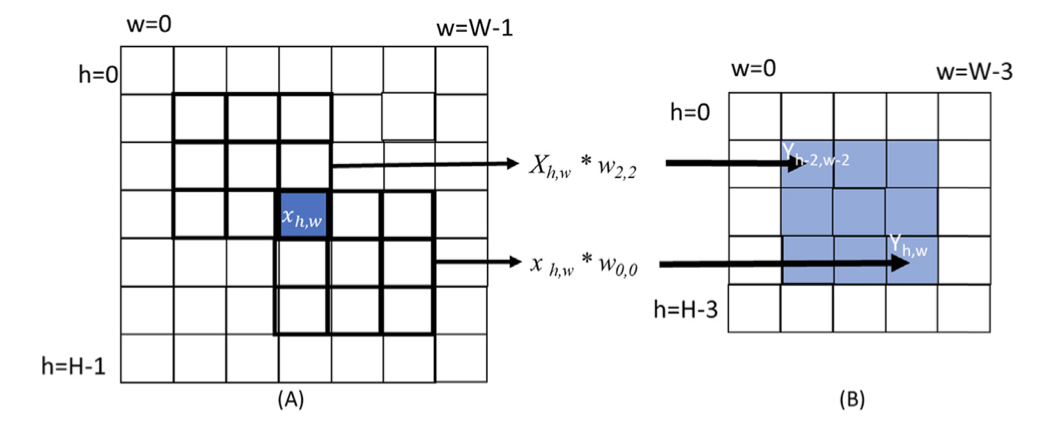
\includegraphics[width=0.9\textwidth]{figs/F16.9.png}
	\caption{\textit{使用硬件线程将线程映射到Kernel }}
\end{figure}

与环境变量 DPCPP\_CPU\_CU\_AFFINITY 结合使用,还有其他支持 CPU 性能调优的环境变量:

\begin{itemize}
	\item DPCPP\_CPU\_NUM\_CUS = [n],设置用于Kernel执行的线程数。 它的默认值是系统中硬件线程的数量。

	\item DPCPP\_CPU\_PLACES = [ sockets| numa\_domains | numa\_domains | cores| threads ],
	它指定将设置关联性的位置,类似于 OpenMP 5.1 中的 OMP\_PLACES。 默认设置是核心。

	\item DPCPP\_CPU\_SCHEDULE = [ dynamic| affinity| static ],指定调度工作组的算法。 
	它的默认设置是动态的。
	
	dynamic:启用auto\_partitioner,它通常会执行足够的分割以平衡工作线程之间的负载。

	affinity:启用affinity\_partitioner,它可以提高缓存亲和力,并在将子范围映射到工作线程时使用比例分割。

	static:启用 static\_partitioner,它尽可能均匀地在工作线程之间分配迭代。
\end{itemize}


当使用 Intel 的 OpenCL CPU 运行时在 CPU 上运行时,工作组调度由线程构建块 (TBB) 库处理。 
使用 DPCPP\_CPU\_SCHEDULE 确定使用哪个 TBB 分区程序。 
请注意,TBB 分区程序还使用粒度大小来控制工作拆分,默认粒度大小为 1,这表示所有工作组都可以独立执行。 
更多信息请访问tinyurl.com/oneTBBpart。

缺乏线程亲和性调整并不一定意味着性能较低。 
性能通常更多地取决于并行执行的线程总数,而不是线程和数据的关联和绑定程度。 
使用基准测试应用程序是确定线程关联是否对性能产生影响的一种方法。 
STREAM Triad 代码如图 16-1 所示,在没有线程关联设置的情况下,一开始性能较低。 
通过控制亲和力设置并通过环境变量使用软件线程的静态调度(Linux 的导出如下所示),性能得到了提高:

export DPCPP\_CPU\_PLACES=numa\_domains 

export DPCPP\_CPU\_CU\_AFFINITY=close

通过使用 numa\_domains 作为亲和性的场所设置,TBB 任务区域绑定到 NUMA 节点或套接字,
并且工作均匀分布在任务区域之间。 
一般来说,环境变量DPCPP\_CPU\_PLACES建议与DPCPP\_CPU\_CU\_AFFINITY一起使用。 
这些环境变量设置帮助我们在具有 2 个插槽、每个插槽 28 个Kernel、
每个Kernel 2 个硬件线程、运行频率为 2.5 GHz 的 Intel Xeon 服务器系统上实现约 30\% 的性能增益。 
不过,我们仍然可以做得更好,进一步提高这款CPU的性能。

\subsubsection{注意第一次接触内存}
内存存储在第一次接触(使用)的地方。 由于我们示例中的初始化循环是由主机线程串行执行的,
因此所有内存都与主机线程正在其上运行的套接字相关联。 
其他套接字的后续访问将从附加到初始套接字(用于初始化)的内存中访问数据,这对于性能来说显然是不受欢迎的。 
我们可以通过并行化初始化循环来控制跨套接字的首次触摸效果,
从而在 STREAM Triad Kernel上实现更高的性能,如图 16-10 所示。

\begin{figure}[H]
	\centering
	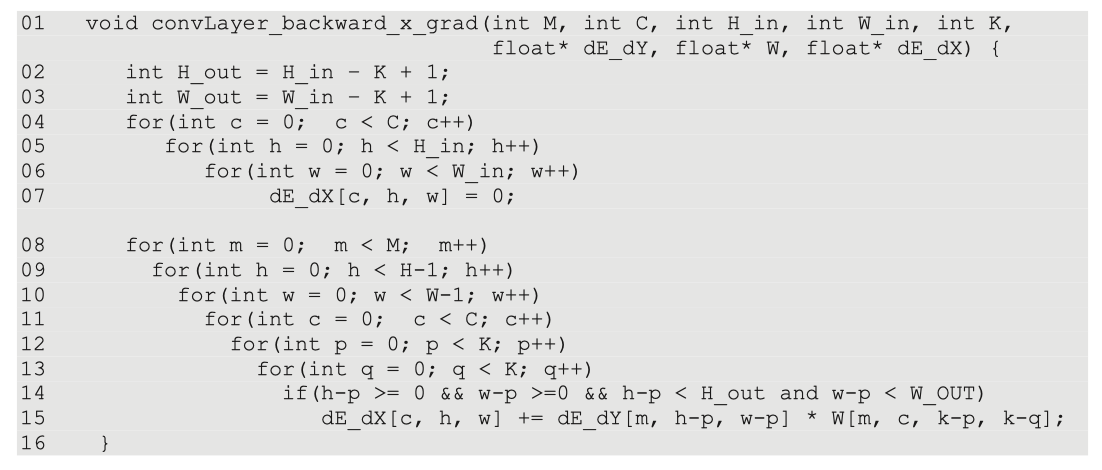
\includegraphics[width=0.9\textwidth]{figs/F16.10.png}
	\caption{\textit{STREAM Triad 并行初始化Kernel,用于控制首次触摸效果 }}
\end{figure}

在初始化代码中利用并行性可以提高Kernel在 CPU 上运行时的性能。 
在本例中,我们在 Intel Xeon 处理器系统上实现了约 2 倍的性能提升。

本章最近的部分表明,通过利用线程级并行性,我们可以有效地利用 CPU Kernel和线程。 
然而,我们还需要利用 CPU 核心硬件中的 SIMD 矢量级并行性来实现峰值性能。

\begin{remark}
	SYCL 并行Kernel受益于跨Kernel和硬件线程的线程级并行性!
\end{remark}

\subsection{CPU 上的 SIMD 矢量化}
虽然编写良好且没有跨工作项依赖性的 SYCL Kernel可以在 CPU 上有效地并行运行,
但实现也可以将矢量化应用于 SYCL Kernel,以利用类似于第 15 章中描述的 GPU 支持的 SIMD 硬件。
本质上,CPU 处理器可以 利用大多数数据元素通常位于连续内存中并通过数据并行Kernel采用相同控制流路径的事实,
使用 SIMD 指令优化内存加载、存储和操作。 
例如,在具有语句 a[i] = a[i] + b[i] 的Kernel中,
每个数据元素通过在多个数据元素之间共享硬件逻辑来执行相同的指令流加载、加载、添加和存储,
并且 将它们作为一个组执行,这可以自然地映射到硬件的 SIMD 指令集上。 
具体地,可以通过单个指令同时处理多个数据元素。

\begin{figure}[H]
	\centering
	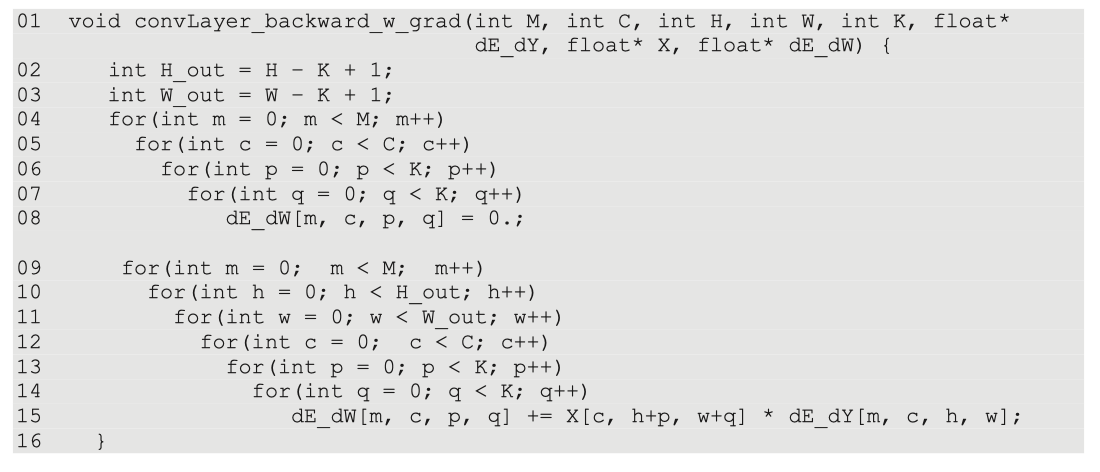
\includegraphics[width=0.9\textwidth]{figs/F16.11.png}
	\caption{\textit{SIMD 执行指令流 }}
\end{figure}

单个指令同时处理的数据元素的数量有时称为指令或执行该指令的处理器的向量长度(或 SIMD 宽度)。 
在图 16-11 中,我们的指令流以四路 SIMD 执行方式运行。

CPU 处理器并不是唯一实现 SIMD 指令集的处理器。 GPU 等其他处理器实现 SIMD 指令以提高处理大量数据时的效率。 
与其他处理器类型相比,Intel Xeon CPU 处理器的一个关键区别在于具有三个固定大小的 SIMD 寄存器宽度(
128 位 XMM、256 位 YMM 和 512 位 ZMM),而不是可变长度的 SIMD 宽度。 
当我们使用Sub-Groups或向量类型编写具有 SIMD 并行性的 SYCL 代码时(请参阅第 11 章),
我们需要注意硬件中 SIMD 宽度和 SIMD 向量寄存器的数量。

\subsubsection{确保SIMD执行合法性}
从语义上讲,SYCL执行模型确保SIMD执行可以应用于任何Kernel,
并且每个工作组(即Sub-Groups)中的一组工作项可以使用SIMD指令同时执行。 
某些实现可能会选择使用 SIMD 指令在Kernel中执行循环,但当且仅当保留所有原始数据依赖性,
或者编译器基于私有化和归约语义解决数据依赖性时,这才是可能的。 这种实现可能会报告Sub-Groups大小为 1。

单个 SYCL Kernel执行可以从处理单个工作项转换为使用工作组内的 SIMD 指令处理一组工作项。 
在 ND 范围模型下,编译器矢量化器会选择增长最快(单位步长)的维度来生成 SIMD 代码。 
本质上,要在给定 ND 范围的情况下启用矢量化,同一Sub-Groups中的任何两个工作项之间不应存在跨工作项依赖关系,
或者编译器需要在同一Sub-Groups中保留跨工作项前向依赖关系。 Sub-Groups。

\begin{figure}[H]
	\centering
	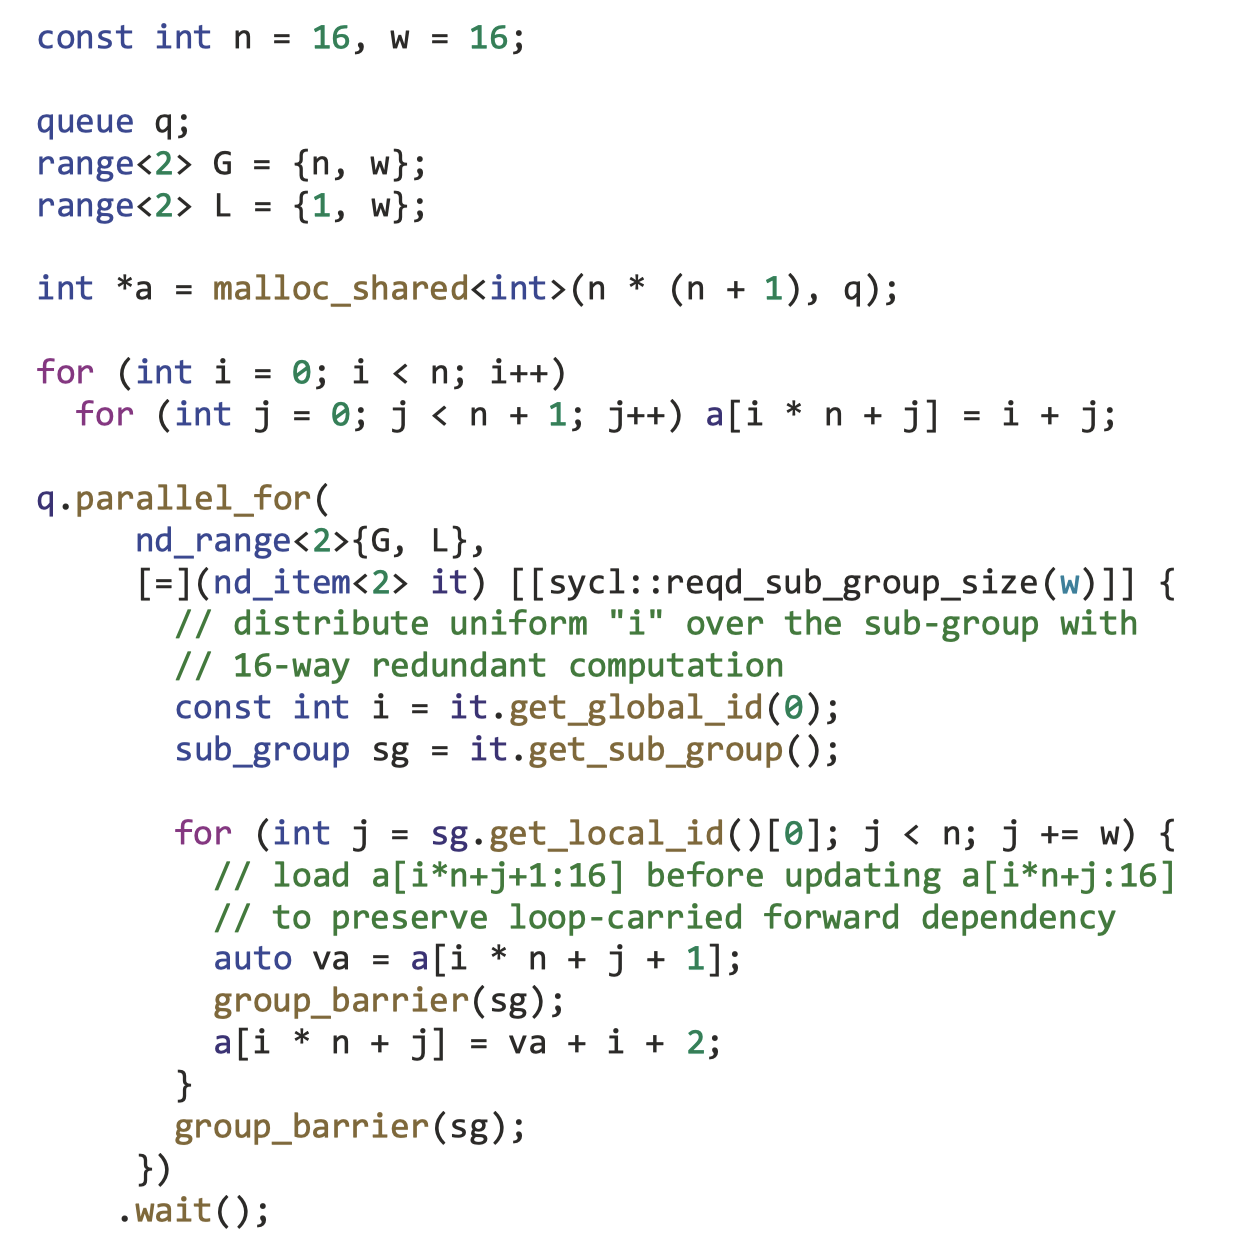
\includegraphics[width=0.9\textwidth]{figs/F16.12.png}
	\caption{\textit{使用Sub-Groups对具有前向依赖关系的循环进行矢量化 }}
\end{figure}

当工作项的Kernel执行映射到 CPU 上的线程时,细粒度同步的成本很高,而且线程上下文切换开销也很高。 
因此,在为CPU编写SYCLKernel时,消除工作组内工作项之间的依赖性是一项重要的性能优化。 
另一种有效的方法是将这种依赖性限制在Sub-Groups内的工作项,如图 16-12 中的先读后写依赖性所示。 
如果Sub-Groups在SIMD执行模型下执行,
则Kernel中的Sub-Groups屏障可以被编译器视为noop,并且在运行时不会产生真正的同步成本。

\begin{figure}[H]
	\centering
	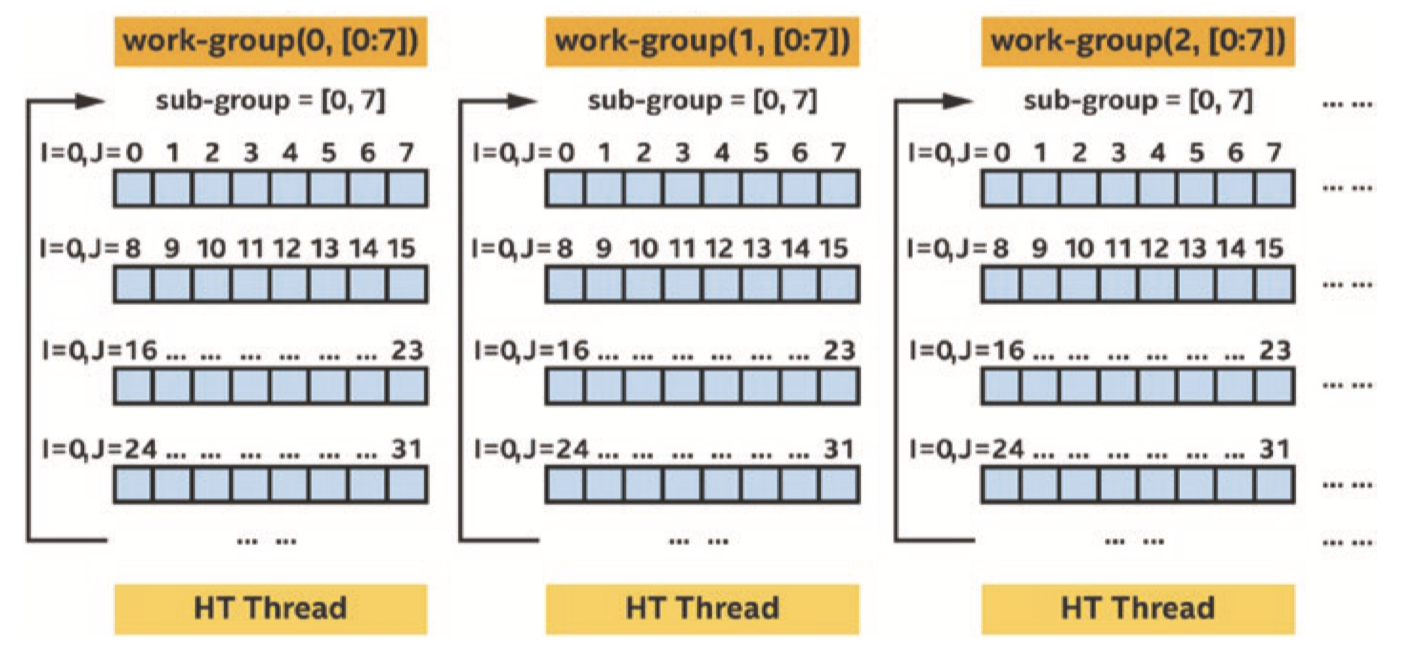
\includegraphics[width=0.9\textwidth]{figs/F16.13.png}
	\caption{\textit{具有前向依赖关系的循环的 SIMD 矢量化 }}
\end{figure}

Kernel被向量化(以向量长度为8为例),其SIMD执行如图16-13所示。 
工作组的组大小为 (1, 8),Kernel内部的循环迭代分布在这些Sub-Groups工作项上,并以八路 SIMD 并行方式执行。

在此示例中,如果Kernel中的循环主导性能,则允许跨Sub-Groups进行 SIMD 矢量化将带来显着的性能改进。

使用并行处理数据元素的 SIMD 指令是让Kernel性能超越 CPU 核心和硬件线程数量的一种方法。

\subsubsection{SIMD 掩蔽和成本}
在实际应用中,我们可以期待条件语句,例如 if 语句,条件表达式,
例如 a = b > a? a: b、具有可变迭代次数的循环、switch 语句等。 
任何有条件的事情都可能导致标量控制流不执行相同的代码路径,就像在 GPU 上一样(第 15 章)可能会导致性能下降。 
SIMD 掩码是一组值为 1 或 0 的位,由Kernel中的条件语句生成。 
考虑一个示例,其中 A={1, 2, 3, 4},B={3, 7, 8, 1} 以及比较表达式 a < b。 
比较返回一个具有四个值 {1, 1, 1, 0} 的掩码,这些值可以存储在硬件掩码寄存器中,
以指示后续 SIMD 指令的哪些通道应执行由比较保护(启用)的代码。

如果Kernel包含条件代码,则会使用基于与每个数据元素(SIMD 指令中的通道)关联的掩码位执行的掩码指令对其进行矢量化。 
每个数据元素的掩码位是掩码寄存器中的相应位。

使用屏蔽可能会导致性能低于相应的非屏蔽代码。 这可能是由于

\begin{itemize}
	\item 每个负载上的附加蒙版混合操作

	\item 对目的的依赖
\end{itemize}

屏蔽是有成本的,因此仅在必要时使用。 当Kernel是 ND 范围Kernel且在执行范围内具有显式工作项分组时,
在选择 ND 范围工作组大小时应小心,以通过最小化屏蔽成本来最大化 SIMD 效率。 
当工作组大小不能被处理器的 SIMD 宽度整除时,部分工作组可能会在Kernel屏蔽的情况下执行。

\begin{figure}[H]
	\centering
	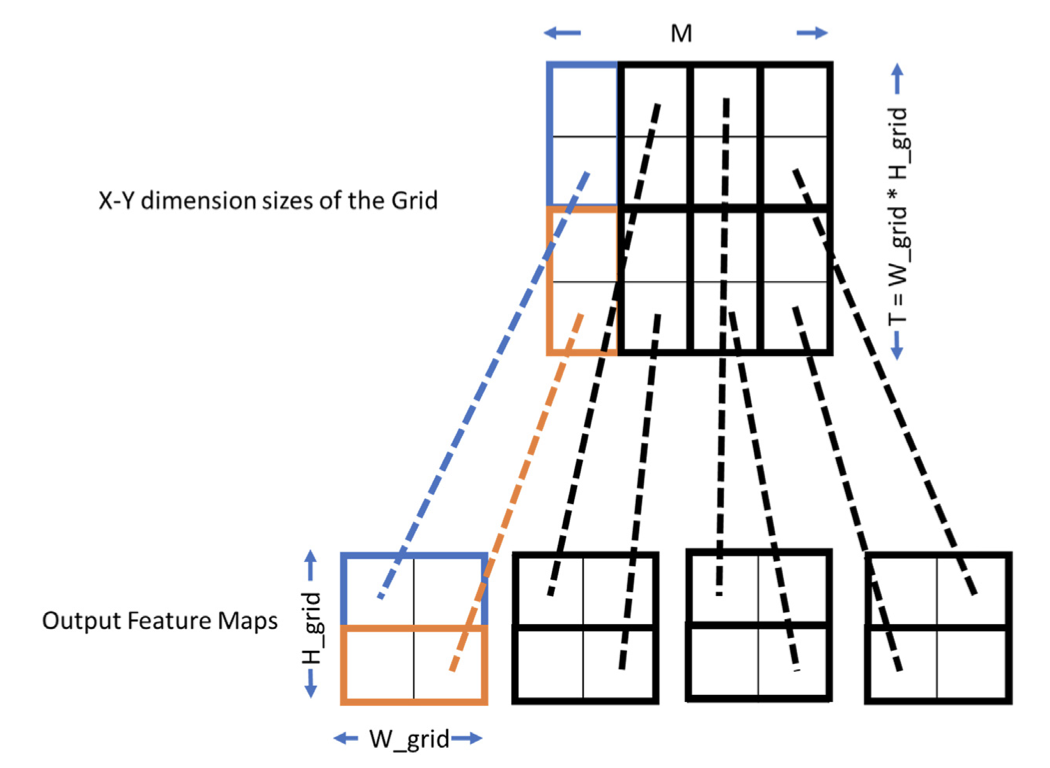
\includegraphics[width=0.9\textwidth]{figs/F16.14.png}
	\caption{\textit{用于Kernel中屏蔽的三个屏蔽代码生成 }}
\end{figure}

图 16-14 显示了使用合并屏蔽如何创建对目标寄存器的依赖:

\begin{itemize}
	\item 在没有屏蔽的情况下,处理器每个周期执行两次乘法(vmulps)。

	\item 通过合并掩码,处理器每四个周期执行两次乘法,因为乘法指令(vmulps) 将结果保存在目标寄存器中,
	如图16-17 所示。

	\item 零掩码不依赖于目标寄存器,因此每个周期可以执行两次乘法(vmulps)。
\end{itemize}

访问缓存对齐的数据比访问未对齐的数据具有更好的性能。 在许多情况下,地址在编译时未知,或者已知但未对齐。 
当使用循环时,可以实现存储器访问的剥离,以使用掩码访问处理前几个元素,
直到第一个对齐地址,然后通过多版本技术处理未掩码访问,然后处理掩码剩余部分。 
此方法增加了代码大小,但总体上改进了数据处理。 
当使用并行Kernel时,我们作为程序员可以通过手动采用类似的技术或通过确保分配适当对齐来提高性能。

\subsubsection{避免结构数组以提高 SIMD 效率}
AOS(结构数组)结构会导致聚集和分散,这既会影响 SIMD 效率,也会为内存访问带来额外的带宽和延迟。 
硬件收集-分散机制的存在并不能消除这种转换的需要——收集-分散访问通常需要比连续负载高得多的带宽和延迟。 
给定 struct \{float x; float y; float z; float w;\} a[4]
考虑一个对其进行操作的Kernel,如图 16-15 所示。

\begin{figure}[H]
	\centering
	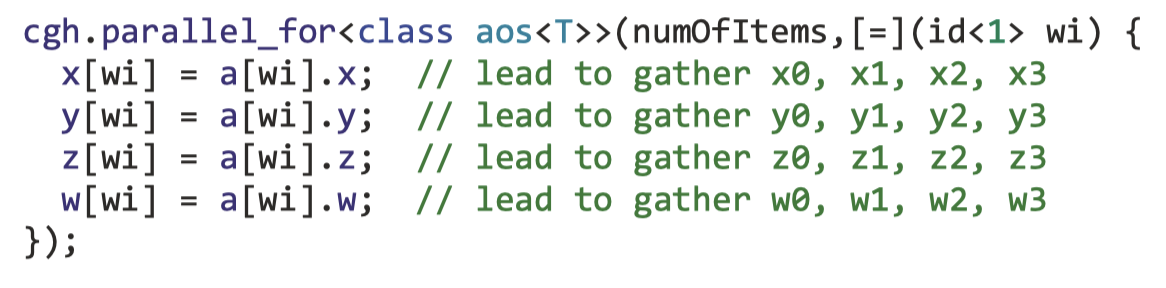
\includegraphics[width=0.9\textwidth]{figs/F16.15.png}
	\caption{\textit{Kernel中的SIMD gather }}
\end{figure}

当编译器沿着一组工作项对Kernel进行矢量化时,由于需要非单位跨度内存访问,它会导致 SIMD 收集指令生成。 
例如,a[0].x、a[1].x、a[2].x 和 a[3].x 的步长是 4,而不是更有效的单位步长 1。

\begin{figure*}[!htbp]
	\centering
	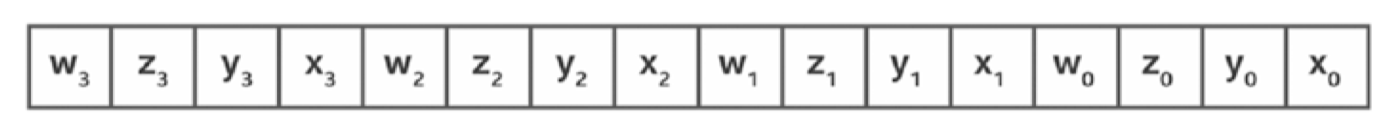
\includegraphics[width=0.9\textwidth]{figs/F16-a1.png}
\end{figure*}

在Kernel中,我们通常可以通过消除内存聚集-分散操作来实现更高的 SIMD 效率。 
某些代码受益于数据布局更改,该更改将以结构数组 (AOS) 表示形式编写的数据结构转换为数组结构 (SOA) 表示形式,
即为每个结构字段使用单独的数组以保留内存访问 执行 SIMD 矢量化时是连续的。 
例如,考虑 struct \{float x[4]; float y[4]; float z[4]; float w[4];\} a; 的 SOA 数据布局, 如图所示:

\begin{figure*}[!htbp]
	\centering
	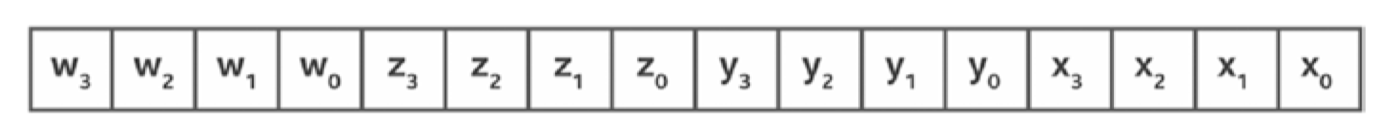
\includegraphics[width=0.9\textwidth]{figs/F16-a2.png}
\end{figure*}

Kernel可以使用单位步长(连续)向量加载和存储来操作数据,如图 16-16 所示,即使是向量化时也是如此!

\begin{figure}[H]
	\centering
	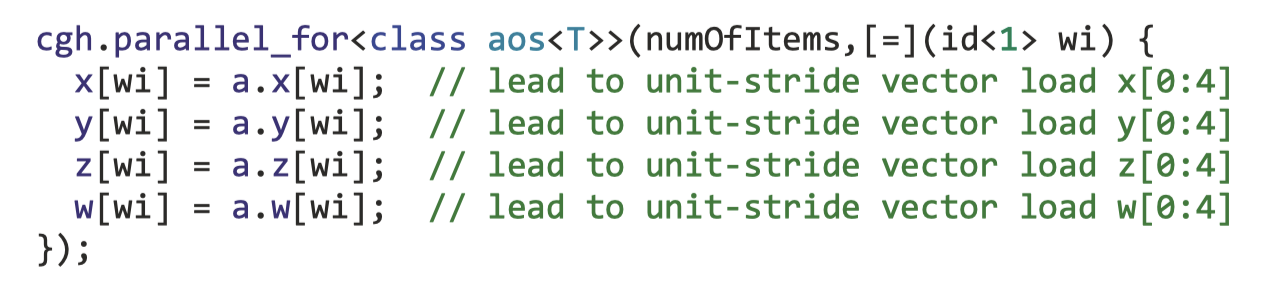
\includegraphics[width=0.9\textwidth]{figs/F16.16.png}
	\caption{\textit{Kernel中的 SIMD 单位步幅向量负载 }}
\end{figure}

SOA 数据布局有助于防止跨数组元素访问结构的一个字段时发生聚集,
并帮助编译器在与工作项关联的连续数组元素上对Kernel进行矢量化。 
请注意,考虑到使用这些数据结构的所有位置,此类 AOS 到 SOA 或 AOSOA 数据布局转换预计将在程序级别(由我们)完成。 
仅在循环级别执行此操作将涉及循环之前和之后格式之间的昂贵转换。 
然而,我们也可能依赖编译器对 AOS 数据布局执行向量加载和洗牌优化,但需要付出一些代价。 
当SOA(或AOS)数据布局的成员具有向量类型时,编译器向量化可以根据底层硬件进行水平扩展或垂直扩展以生成最优代码。

\subsubsection{数据类型对 SIMD 效率的影响}
当 C++ 程序员知道数据适合 32 位有符号类型时,他们通常会使用整数数据类型,这通常会导致如下代码

int id = get\_global\_id(0); a[id] = b[id] + c[id];

但是,鉴于 get\_global\_id(0) 的返回类型是 size\_t(无符号整数,通常是 64 位),
转换可能会减少编译器可以合法执行的优化。 当编译器对Kernel中的代码进行矢量化时,
这可能会导致 SIMD 收集/分散指令,例如:

\begin{itemize}
	\item 读取[get\_global\_id(0)] 可能会导致SIMD 单位步长向量加载。

	\item 读取[(int)get\_global\_id(0)] 可能会导致非单位步长收集指令。
\end{itemize}

这种微妙的情况是由从 size\_t 到 int (或 uint)的数据类型转换的环绕行为
(C++ 标准中未指定的行为和/或明确定义的环绕行为)引入的,这主要是基于 C 语言的演变的历史产物。 
具体来说,某些转换的溢出是未定义的行为,这允许编译器假设此类情况永远不会发生并更积极地进行优化。 
图 16-17 为那些想要了解细节的人展示了一些示例。

\begin{figure}[H]
	\centering
	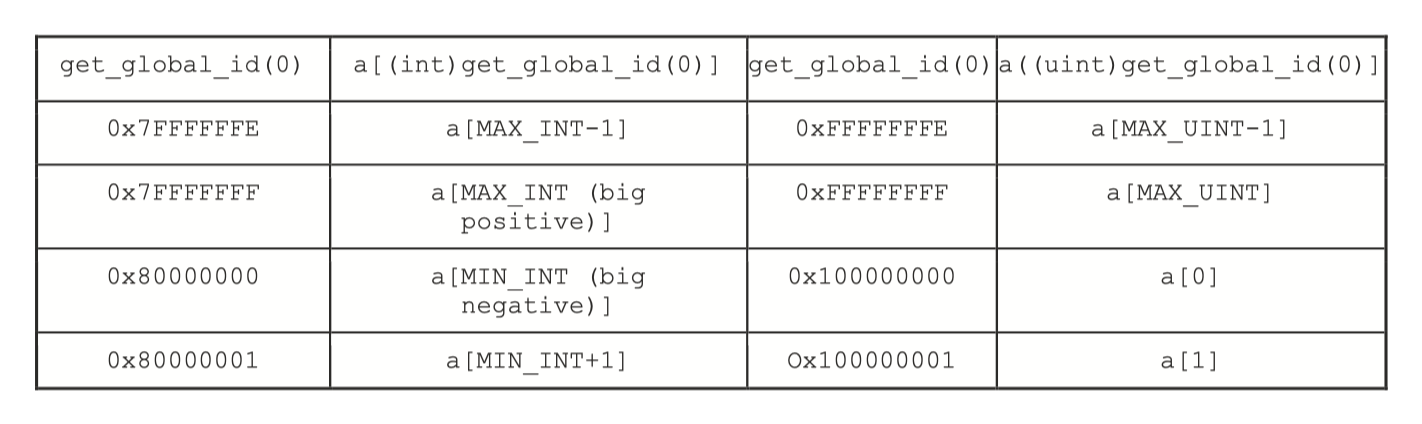
\includegraphics[width=0.9\textwidth]{figs/F16.17.png}
	\caption{\textit{整数类型的value wrapper around }}
\end{figure}

SIMD 聚集/分散指令比 SIMD 单位步长向量加载/存储操作慢。 
为了实现最佳的 SIMD 效率,无论使用哪种编程语言,避免聚集/分散对于应用程序都是至关重要的。

大多数 SYCL get\_*\_id() 系列函数具有相同的细节,
尽管许多情况适合 MAX\_INT,因为可能的返回值是有限的(例如,工作组内的最大 id)。 
因此,只要合法,SYCL 编译器就可以假定跨相邻工作项块的单位步长内存地址,以避免聚集/分散。 
如果由于全局 ID 的值和/或全局 ID 的导数值可能溢出而导致编译器无法安全地生成线性单位步长向量内存加载/存储,
则编译器将生成聚集/分散。

在为用户提供最佳性能的理念下,DPC++编译器假设没有溢出,并且在实践中几乎所有时间都捕捉到了现实,
因此编译器可以生成最佳的SIMD代码以实现良好的性能。 
然而,DPC++编译器为我们提供了一个编译器选项-fnosycl-id-queries-fit-in-int,
告诉编译器将会出现溢出,并且从id查询派生的向量化访问可能不安全。 这可能会对性能产生很大的影响,
并且应该在不安全的情况下使用,以假设没有溢出。 关键要点是程序员应确保全局 ID 的值适合 32 位 int。 
否则,应使用编译器选项 -fno-sycl-idqueries-fit-in-int 来保证程序的正确性,这可能会导致性能降低。

\subsubsection{使用 single\_task 执行 SIMD}
在单任务执行模型下,没有要矢量化的工作项。 与向量类型和函数相关的优化是可能的,但这取决于编译器。 
编译器和运行时可以自由地启用显式 SIMD 执行或在 single\_task Kernel中选择标量执行,结果将取决于编译器的实现。

当编译到 CPU 时,C++ 编译器可能会将 single\_task 内部出现的向量类型映射到 SIMD 指令。 
vec load、store 和 swizzle 函数直接对向量变量执行操作,
通知编译器数据元素正在从内存中的同一(统一)位置开始访问连续数据,并使我们能够请求连续数据的优化加载/存储。 
正如第 11 章中所讨论的,这种对 vec 的解释是有效的,
但是,我们应该预期该功能最终会被弃用,而支持更明确的向量类型(例如,std::simd)。

\begin{figure}[H]
	\centering
	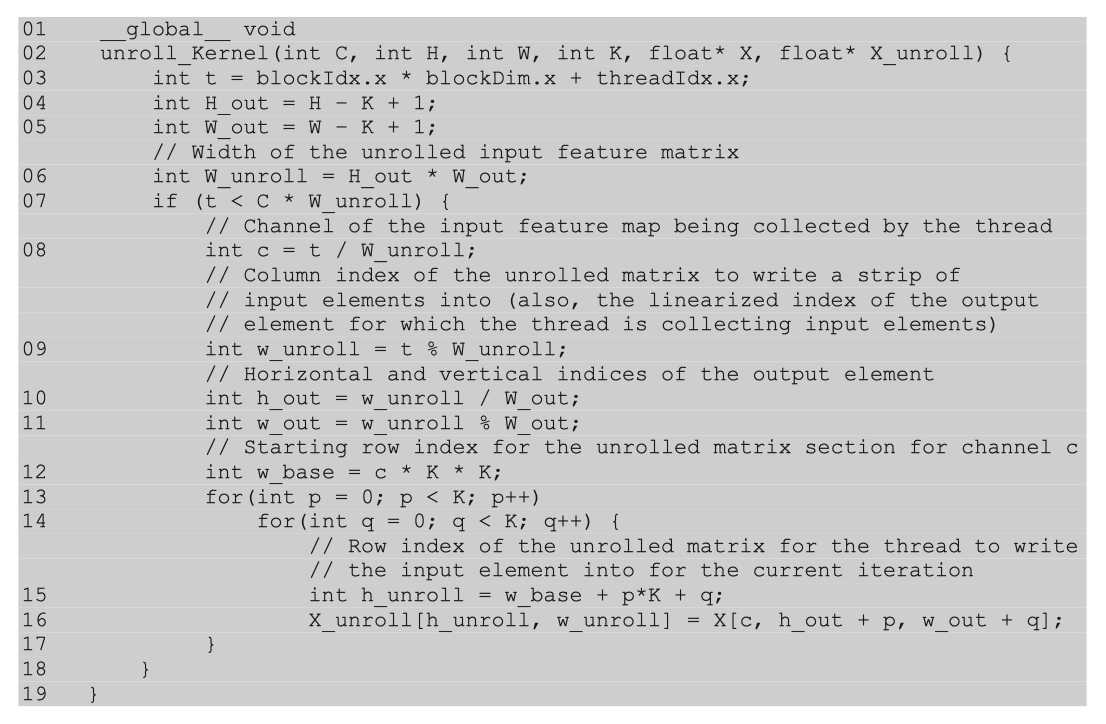
\includegraphics[width=0.9\textwidth]{figs/F16.18.png}
	\caption{\textit{在single\_taskKernel中使用向量类型和 swizzle 操作 }}
\end{figure}

在图16-18所示的示例中,在单任务执行下,声明了一个具有三个数据元素的向量。 
使用 old\_v.abgr() 执行 swizzle 操作。 如果 CPU 为某些 swizzle 操作提供 SIMD 硬件指令,
我们可以通过在应用程序中使用 swizzle 操作来实现一些性能优势。

\begin{remark}[SIMD 矢量化指南]
CPU 处理器实现具有不同 SIMD 宽度的 SIMD 指令集。
在许多情况下,这是一个实现细节,对于在 CPU 上执行Kernel的应用程序是透明的,
因为编译器可以确定一组有效的数据元素,以特定的 SIMD 大小进行处理,而不是要求我们显式使用 SIMD 指令。
Sub-Groups可用于更直接地表示数据元素分组应在Kernel中执行 SIMD 的情况。

考虑到计算的复杂性,选择最适合矢量化的代码和数据布局最终可能会带来更高的性能。
在选择数据结构时,请尝试选择数据布局、对齐方式和数据宽度,
以便最常执行的计算能够以具有最大并行度的 SIMD 友好方式访问内存,如本章所述。
\end{remark}

\subsection{总结}
为了充分利用 CPU 上的线程级并行性和 SIMD 矢量级并行性,我们需要牢记以下目标:

\begin{itemize}
	\item 熟悉所有类型的SYCL 并行性以及我们希望针对的底层CPU 架构。

	\item 在最匹配硬件资源的线程级别利用适量的并行性(不多也不少)。 
	使用分析器和分析器等供应商工具来帮助指导我们的调优工作以实现这一目标。

	\item 注意线程亲和性和内存首次接触对程序性能的影响。

	\item 通过数据布局、对齐方式和数据宽度来设计数据结构,
	以便最常执行的计算能够以SIMD 友好的方式访问内存,并具有最大的SIMD 并行性。

	\item 注意平衡屏蔽与代码分支的成本。

	\item 使用清晰的编程风格,最大限度地减少潜在的内存别名和副作用。

	\item 请注意使用向量类型和接口的可扩展性限制。 
	如果编译器实现将它们映射到硬件 SIMD 指令,
	则固定向量大小可能无法在多代 CPU 和来自不同供应商的 CPU 中很好地匹配 SIMD 寄存器的 SIMD 宽度。
\end{itemize}